
\chapter{Counting}

If the title of this chapter seems less than inspiring, it's only because
the kind of counting we learned as children was mostly of a straightforward
kind. In this chapter, we're going to learn to answer some more difficult
questions like ``how many different semester schedules could a college
student possibly have?" and ``how many different passwords can a
customer choose for this e-commerce website?" and ``how likely is this
network buffer to overflow, given that its packets are addressed to three
different destinations?"

\index{combinatorics}
\index{enumerating}
The more impressive-sounding name for this topic is \textbf{combinatorics}.
In combinatorics, we focus on two tasks: counting things (to find out how
many there are), and enumerating things (to systematically list them as
individuals). Some things turn out to be hard to count but easy to
enumerate, and vice versa.

\section{The Fundamental Theorem}

\index{Fundamental Theorem of Counting}
We start with a basic rule that goes by the audacious name of \textbf{The
Fundamental Theorem of Counting}.\footnote{How many other ``Fundamental
Theorems" of math do you know? Here are a few: the Fundamental Theorem of
Arithmetic says that any natural number can be broken down into its prime
factors in only one way. The Fundamental Theorem of Algebra says that the
highest power of a polynomial is how many roots (zeroes) it has. The
Fundamental Theorem of \textit{Linear} Algebra says that the row space and the
column space of a matrix have the same dimension. The Fundamental Theorem of
Calculus says that integration and differentiation are the inverse of each
other.} It goes like this:

\begin{nobreak}

\fbox{\parbox{\textwidth}{If a whole can be divided into $k$ parts, and
there's $n_i$ choices for the $i^{\text{th}}$ part, then there's $n_1
\times n_2 \times n_3 \times \cdots \times n_k$ ways of doing the whole
thing.}}

\end{nobreak}

Example: Jane is ordering a new Lamborghini. She has twelve different
paint colors to choose from (including Luscious Red and Sassy Yellow),
three different interiors (Premium Leather, Bonded Leather, or Vinyl), and
three different stereo systems. She must also choose between automatic and
manual transmission, and she can get power locks \& windows (or not). How
many different configurations does Jane have to choose from? Put another
way, how many different kinds of cars could come off the line for her?

The key is that every one of her choices is independent of all the others.
Choosing an Envious Green exterior doesn't constrain her choice of
transmission, stereo, or anything else. So no matter which of the 12 paint
colors she chooses, she can independently choose any of the three
interiors, and no matter what these first two choices were, she can freely
choose any of the stereos, \textit{etc.} It's a mix-and-match. Therefore
the answer is:

\[
12 \times 3 \times 3 \times 2 \times 2 = 432\ \text{choices}.
\]

Here's an alternate notation you'll run into for this, by the way:

\index{product operator ($\Pi$)}
\[
\prod_{i=1}^k{n_i}
\]
which is just a shorter way of writing
\[
n_1 \times n_2 \times n_3 \times \cdots \times n_k.
\]

\index{summation operator ($\Sigma$)}
As mentioned in section~\ref{totalprob}, the $\Sigma$ notation is
essentially a loop with a counter, and it says to add up the expression to
the right of it for each value of the counter. The $\Pi$ notation is
exactly the same, only instead of adding the expressions together for each
value of the counter, we're multiplying them. (The reason mathematicians
chose the symbols $\Sigma$ (sigma) and $\Pi$ (pi) for this, by the way, is
that ``sigma" and ``pi" start with the same letter as ``sum" and
``product," respectively.)

\index{ATM machines}
\index{PINs}
We can actually get a lot of leverage just with the fundamental theorem.
How many different PINs are possible for an ATM card? There are four
digits, each of which can be any value from 0 to 9 (ten total values), so
the answer is:

\[
10 \times 10 \times 10 \times 10 = 10,000\ \text{different PINs}.
\]

So a thief at an ATM machine frantically entering PINs at random (hoping to
break your account before you call and stop your debit card) would have to
try about 5,000 of them on average before cracking the code.

\index{locker combinations}
What about middle school bullies who are trying to break into your locker?
Well, most combination locks are opened by a three-number sequence, each
number of which is anything from 0 to 39. So there are:

\[
40 \times 40 \times 40 = 64,000\ \text{different combinations}.
\]

That's probably slightly overstated, since I'll bet consecutive repeat
numbers are not allowed (Master probably doesn't manufacture a lock with a
combination of 17--17--23, for example.) But it does seem at least as
secure as a PIN number.

\index{license plates}
Every car in the state of Virginia must be issued its own license plate
number. That's a lot of cars. How many different license plate combinations
are available?

This one requires a bit more thought, since not all licenses numbers have
the same number of characters. In addition to ``\texttt{SED4756}" and
``\texttt{PXY1927}" you can also have ``\texttt{DAWG}" or ``\texttt{LUVME}"
or even ``\texttt{U2}". How can we incorporate these?

\index{mutually exclusive}
The trick is to divide up our set into mutually exclusive subsets, and then
add up the cardinalities of the subsets. If only 7 characters fit on a
license plate, then clearly every license plate number has either 1, 2, 3,
4, 5, 6, or 7 characters. And no license plate has \textit{two} of these
(\textit{i.e.}, there is no plate that is both 5 characters long
\textit{and} 6 characters long). Therefore they're mutually exclusive
subsets, and safe to add. This last point is often not fully appreciated,
leading to errors. Be careful not to cavalierly add the cardinalities of
non-mutually-exclusive sets! You'll end up double-counting items.

So we know that the number of possible license plates is equal to:
\begin{center}
the \# of 7-character plates + \\
the \# of 6-character plates + \\
the \# of 5-character plates + \\
$\cdots$ + \\
the \# of 1-character plates.
\end{center}

Very well. We can now figure out each one separately. How do we know how
many 7-character plates there are? Well, if every character must be either
a letter or a digit, then we have 26 + 10 = 36 choices for each character.
This implies $36^7$ different possible 7-character license plates. The
total number of plates is therefore:
\[
36^7 + 36^6 + 36^5 + 36^4 + 36^3 + 36^2 + 36 = \text{80,603,140,212 plates}
\]

which is about ten times the population of the earth, so I think we're
safe for now.

Here's an interesting thought experiment to test your intuition about
numbers. Look at the above calculation, and ask yourself: ``what if the
state of Virginia decided, for purposes of consistency, that all license
plates \textit{had} to have the full 7 characters? Would that significantly
reduce the total number of possible plates?" My first inclination would be
to say ``yes," because we're adding seven things in that equation, and if
we mandated 7-character plates for everyone we'd eliminate 6 out of the 7.
Surely we'd be in danger of running out of license plates to give to all
the cars! But in fact the new total number of plates would turn out to be:
\[
36^7 = \text{78,364,164,096 plates}.
\]

\index{exponential growth}
Wow. We've hardly lost \textit{anything} by scrapping all the
less-than-7-character plates. Turns out that in comparison with the
7-character plates, all the other lengths were a drop in the bucket. This
is a powerful illustration of exponential growth. When you modify the
exponent, going from something like $36^6$ to $36^7$, you get
astronomically larger very, very quickly. This is a good thing to know when
all you want is an approximation of some quantity. How many passwords are
possible in a system that mandates 6-10 characters per password? Well, you
can pretty much ignore all the 6-9 character passwords and just count the
10-character passwords, because there are so many more of those.

One last tweak to the license plate example before we move on. Suppose
(again, for the sake of consistency) that Virginia outlawed personalized
plates and gave everyone a randomly generated 7-character plate.
Furthermore, the last four characters of the plate had to be
\textit{digits} instead of letters, so that something like
``\text{RFP-6YQ7}" would be impossible. Now how many possible plates would
there be?

In this case, not each of the $k$ parts of $n$ have an equal number of
choices. $n_1$ through $n_3$ are still 36, but now $n_4$ through $n_7$ are
just 10. So this gives us:
\[
36 \times 36 \times 36 \times 10 \times 10 \times 10 \times 10 =\ 
\text{466,560,000 plates}
\]

or only about .006 times as many as before. Better stick with alphanumeric
characters for all seven positions.


\subsubsection{A simple trick}

\index{complement, total (of sets)}
Sometimes we have something difficult to count, but we can turn it around
in terms of something much easier. Often this involves counting the
\textit{complement} of something, then subtracting from the total.

\index{passwords}
For instance, suppose a certain website mandated that user passwords be
between 6-10 characters in length --- every character being an uppercase
letter, lowercase letter, digit, or special character (\texttt{*},
\texttt{\#}, \texttt{@}, \texttt{\%} or \texttt{\&}) --- but it also
required each password to have \textit{at least one digit or special
character.} How many passwords are possible?

Without the ``at least one digit or special character" part, it's pretty
easy: there are 26 + 26 + 10 + 5 = 67 different choices for each character,
so we have
\[
67^{10} + 67^9 + 67^8 + 67^7 + 67^6 = \text{1,850,456,557,795,600,384
strings}.
\]

But how do we handle the ``at least one" part?

One way would be to list all the possible ways of having a password with at
least one non-alpha character. The non-alpha could appear in the first
position, or the second, or the third, $\dots$, or the tenth, but of course
this only works for 10-digit passwords, and in any event it's not like the
\textit{other} characters couldn't \textit{also} be non-alpha. It gets
messy really fast.

There's a simple trick, though, once you realize that it's easy to count
the passwords that \textit{don't} satisfy the extra constraint. Ask
yourself this question: out of all the possible strings of 6-10 characters,
how many of them \textit{don't} have at least one non-alpha character? (and
are therefore illegal, according to the website rules?)

It turns out that's the same as asking ``how many strings are there with
6-10 alphabetic (only) characters?" which is of course:
\[
52^{10} + 52^9 + 52^8 + 52^7 + 52^6 = \text{147,389,519,403,536,384
(illegal) passwords}.
\]

Now, all we have to do is subtract to get
{\small
\begin{align*}
\text{total \# of strings -- \# of illegal passwords} & = \text{\# of legitimate passwords} \\
\text{1,850,456,557,795,600,384 -- 147,389,519,403,536,384} &= \text{1,708,735,865,301,022,720}
\end{align*}
}
legitimate passwords. Looks like we don't lose much by requiring the
non-alpha character.

The lesson learned is that if counting the elements in some set involves
accounting for a lot of different sticky scenarios, it's worth a try to
count the elements \textit{not} in the set instead, and see if that's
easier.


\section{Permutations}

\index{permutations}
\index{Davies family}
When we're counting things, we often run into permutations. A
\textbf{permutation} of $n$ distinct objects is an arrangement of them in a
sequence. For instance, suppose all three Davies kids need to brush their
teeth, but only one of them can use the sink at a time. What order will
they brush in? One possibility is Lizzy, then T.J., then Johnny. Another
possibility is T.J., then Lizzy, then Johnny. Another is Johnny, then
Lizzy, then T.J. These are all different permutations of the Davies kids.
Turns out there are six of them (find all 6 for yourself!)

\index{Fundamental Theorem of Counting}
Counting the number of permutations is just a special application of the
Fundamental Theorem of Counting. For the teeth brushing example, we have
$n=3$ different ``parts" to the problem, each of which has $n_i$ choices to
allocate to it. There are three different Davies kids who could brush their
teeth first, so $n_1=3$. Once that child is chosen, there are then
\textit{two} remaining children who could brush second, so $n_2=2$. Then,
once we've selected a first-brusher and a second-brusher, there's only one
remaining choice for the third-brusher, so $n_3=1$. This means the total
number of possible brushing orders is:
\[
3 \times 2 \times 1 = 6.
\]

\index{factorial}
This pattern comes up so much that mathematicians have established a
special notation for it:
\[
n \times (n-1) \times (n-2) \times \cdots \times 1 = n!\
\text{(``$n$-factorial")}
\]

We say there are ``3-factorial" different brushing orders for the Davies
kids. For our purposes the notion of factorial will only apply for
integers, so there's no such thing as 23.46!~or $\pi$!. (In advanced
computer science applications, however, mathematicians sometimes do define
factorial for non-integers.) We also define 0!~to be 1, which might
surprise you.

\index{Jumble\textsuperscript{\textregistered}}
This comes up a heck of a lot. If I give you a jumbled set of letters to
unscramble, like ``\texttt{KRIBS}" (think of the
Jumble\textsuperscript{\textregistered} word game in the newspaper), how
many different unscramblings are there? The answer is 5!, or 120, one of
which is \texttt{BRISK}. Let's say I shuffle a deck of cards before playing
War.\footnote{``War" is a mindless card game which involves no strategy or
decision-making on the part of the players. Once you shuffle the initial
deck, the entire outcome of the game is fixed.} How many different games of
War are there? The answer is 52!, since any of the cards in the deck might
be shuffled on top, then any \textit{but} that top card could be second,
then any \textit{but} those two could be third, \textit{etc.} Ten packets
arrive near-simultaneously at a network router.  How many ways can they be
queued up for transmission? 10!~ways, just like a larger Davies family.

The factorial function grows really, really fast, by the way, even faster
than exponential functions. A five letter word like ``\texttt{BRISK}" has
120 permutations, but ``\texttt{AMBIDEXTROUSLY}" has 87,178,291,200, ten
times the population of the earth. The number of ways to shuffle a deck is
{\footnotesize
\begin{center}
80,658,175,170,944,942,408,940,349,866,698,506,766,127,860,028,660,283,290,685,487,972,352
\end{center}
}
so I don't think my boys will end up playing the same War game twice any
time soon, nor my wife and I the same bridge hand.


\subsection{Enumerating permutations}
\index{enumerating}

We've discovered that there are 120 permutations of \texttt{BRISK}, but how
would we go about listing them all? You can play around with the Davies
kids and stumble upon all 6 permutations, but for larger numbers it's 
harder. We need a systematic way.

\index{recursion}
Two of the easiest ways to enumerate permutations involve recursion. Here's
one:

\index{algorithm}
\begin{nobreak}
\textbf{Algorithm \#1 for enumerating permutations}
\begin{enumerate}
\item Begin with a set of $n$ objects.
    \begin{enumerate}
    \item If $n=1$, there is only one permutation; namely, the object itself.
    \item Otherwise, remove one of the objects, and find the
    permutations of the remaining $n-1$ objects. Then, insert the removed
    object at every possible position, creating another permutation each time.
    \end{enumerate}
\end{enumerate}
\end{nobreak}

As always with recursion, solving a bigger problem depends on solving
smaller problems. Let's start with \texttt{RISK}. We've already discovered
from the toothbrushing example that the permutations of \texttt{ISK} are
\texttt{ISK}, \texttt{IKS}, \texttt{SIK}, \texttt{SKI}, \texttt{KIS}, and
\texttt{KSI}. So to find the permutations of \texttt{RISK}, we insert an
\texttt{R} into \textit{each} possible location for \textit{each} of these
\texttt{ISK}-permutations. This gives us:
\begin{center}
\texttt{\framebox[.1in]{R}ISK} \\
\texttt{I\framebox[.1in]{R}SK} \\
\texttt{IS\framebox[.1in]{R}K} \\
\texttt{ISK\framebox[.1in]{R}} \\
\texttt{\framebox[.1in]{R}IKS} \\
\texttt{I\framebox[.1in]{R}KS} \\
\texttt{IK\framebox[.1in]{R}S} \\
\texttt{IKS\framebox[.1in]{R}} \\
\texttt{\framebox[.1in]{R}SIK} \\
$\cdots$
\end{center}
and so on. Once we have the \texttt{RISK} permutations, we can generate the
\texttt{BRISK} permutations in the same way:
\begin{center}
\texttt{\framebox[.1in]{B}RISK} \\
\texttt{R\framebox[.1in]{B}ISK} \\
\texttt{RI\framebox[.1in]{B}SK} \\
\texttt{RIS\framebox[.1in]{B}K} \\
\texttt{RISK\framebox[.1in]{B}} \\
\texttt{\framebox[.1in]{B}IRSK} \\
\texttt{I\framebox[.1in]{B}RSK} \\
\texttt{IR\framebox[.1in]{B}SK} \\
\texttt{IRS\framebox[.1in]{B}K} \\
\texttt{IRSK\framebox[.1in]{B}} \\
\texttt{\framebox[.1in]{B}RSIK} \\
$\cdots$
\end{center}

Another algorithm to achieve the same goal (though in a different order) is
as follows:

\index{algorithm}
\begin{nobreak}
\textbf{Algorithm \#2 for enumerating permutations}
\begin{enumerate}
\item Begin with a set of $n$ objects.
    \begin{enumerate}
    \item If $n=1$, there is only one permutation; namely, the object itself.
    \item Otherwise, remove each of the objects in turn, and prepend that
    object to the permutations of all the others, creating another permutation
    each time.
    \end{enumerate}
\end{enumerate}
\end{nobreak}

I find this one a little easier to get my head around, but in the end it's
personal preference. The permutations of \texttt{BRISK} are: ``\texttt{B}
followed by all the permutations of \texttt{RISK}, plus \texttt{R} followed
by all the permutations of \texttt{BISK}, plus \texttt{I} followed by all
the permutations of \texttt{BRSK}, \textit{etc.}" So the first few
permutations of a 4-letter word are:
\begin{center}
\texttt{R \ovalbox{I S K}} \\
\texttt{R \ovalbox{I K S}} \\
\texttt{R \ovalbox{S I K}} \\
\texttt{R \ovalbox{S K I}} \\
\texttt{R \ovalbox{K I S}} \\
\texttt{R \ovalbox{K S I}} \\
\texttt{I \ovalbox{R S K}} \\
\texttt{I \ovalbox{R K S}} \\
\texttt{I \ovalbox{S R K}} \\
\texttt{I \ovalbox{S K R}} \\
\texttt{I \ovalbox{K R S}} \\
\texttt{I \ovalbox{K S R}} \\
\texttt{S \ovalbox{R I K}} \\
$\cdots$
\end{center}

Then, for the 5-letter word:
\begin{center}
\texttt{B \ovalbox{R I S K}} \\
\texttt{B \ovalbox{R I K S}} \\
\texttt{B \ovalbox{R S I K}} \\
\texttt{B \ovalbox{R S K I}} \\
\texttt{B \ovalbox{R K I S}} \\
\texttt{B \ovalbox{R K S I}} \\
\texttt{B \ovalbox{I R S K}} \\
\texttt{B \ovalbox{I R K S}} \\
$\cdots$
\end{center}


\subsection{Partial permutations}

\index{partial permutations}
\index{golf}
Sometimes we want to count the permutations of a set, but only want to
choose \textit{some} of the items each time, not all of them. For example,
consider a golf tournament in which the top ten finishers (out of 45) all
receive prize money, with the first place winner receiving the most, the
second place finisher a lesser amount, and so on down to tenth place, who
receives a nominal prize. How many different finishes are possible to the
tournament?

In this case, we want to know how many different orderings of golfers there
are, but it turns out that past tenth place, we don't care what order they
finished in. All that matters is the first ten places. If the top ten are
1.Tiger, 2.Phil, 3.Lee, 4.Rory, $\dots$, and 10.Bubba, then it doesn't
matter whether Jason finished $11^{\text{th}}$ or $45^{\text{th}}$.

It's easy to see that there are 45 possible winners, then for each winner
there are 44 possible second-placers, \textit{etc.}, so that this total
turns out to be:
{\small
\[
45 \times 44 \times 43 \times 42 \times 41 \times 40 \times 39 \times 38
\times 37 \times 36 = \text{11,576,551,623,436,800 finishes}.
\]
}
Each of the finishes is called a \textbf{partial permutation}. It's a
permutation of $k$ items chosen from $n$ total, and is denoted $p_{n,k}$.
The number of such permutations works out to
\[
n \times (n-1) \times (n-2) \times \cdots \times (n-k+1).
\]
The ``$n-k+1$" bit can be confusing, so take your time and think it
through. For the golf tournament case, our highest term was 45 and our
lowest term was 36. This is because $n$ was 45 and $k$ was 10, and so we
only wanted to carry out the multiplication to 36 (not 35), and 36 is
45-10+1.

\index{factorial}
This can be expressed more compactly in a few different ways. First,
we can use factorials to represent it:
\begin{align*}
n \times (n-1) \times (n-2) \times \cdots \times (n-k+1) &= \\
\dfrac{n \times (n-1) \times (n-2) \times \cdots \times 1}{(n-k) \times (n-k-1) \times (n-k-2) \times \cdots \times 1} &= \dfrac{n!}{(n-k)!}.
\end{align*}
\index{product operator ($\Pi$)}
Too, we could use our compact product notation:
\begin{align*}
n \times (n-1) \times (n-2) \times \cdots \times (n-k+1) &= 
\prod_{i=0}^{k-1}{(n-i)}.
\end{align*}
\index{$n$-to-the-$k$-falling operator}
Finally, as with (non-partial) permutations, this comes up so much that
the professionals have invented a special notation for it. It looks like a
power, but has an underline under the exponent:
\begin{align*}
n \times (n-1) \times (n-2) \times \cdots \times (n-k+1) &= 
n^{\underline{k}}.
\end{align*}
\index{Knuth, Donald}
This is pronounced ``$n$-to-the-$k$-falling," and was invented by one of
the most brilliant computer scientists in history, Donald Knuth.

To keep straight what $n^{\underline{k}}$ means, think of it as the same as
plain exponentiation, except that the product diminishes instead of staying
the same. For example, ``17-to-the-$6^{\text{th}}$" is
\[
17^6 = 17 \cdot 17 \cdot 17 \cdot 17 \cdot 17 \cdot 17
\]
but ``17-to-the-$6^{\text{th}}$-falling" is
\[
17^{\underline{6}} = 17 \cdot 16 \cdot 15 \cdot 14 \cdot 13 \cdot 12.
\]
In both cases, you're multiplying the same number of terms, it's just that
in the second case, these terms are ``falling."

\index{movie channel}
Anyway, notation aside, partial permutations abound in practice. A late
night movie channel might show four classic films back to back every
evening. If there are 500 films in the studio's library, how many nightly
TV schedules are possible? Answer: $500^{\underline{4}}$, since there are
500 choices of what to show at 7pm, then 499 choices for 9pm, 498 for 11pm,
and 497 for the 1am late show.

\index{NASCAR}
The fastest 41 auto racers will qualify for Sunday's race, and will be
placed from Pole Position on down depending on their qualifying time. If 60
cars participate in the qualifying heat, then there are
$60^{\underline{41}}$ different possible starting configurations for
Sunday.

\index{middle school}
Middle schoolers entering sixth grade will be assigned a semester schedule
that consists of five ``blocks" (periods), each of which will have one of
thirteen classes (science, math, orchestra, study hall, \textit{etc.}) How
many schedules are possible? You guessed it, $13^{\underline{5}}$. Notice
that this is the correct answer only because no repeats are allowed: we
don't want to schedule any student for American History more than once.  If
a student \textit{could} take the same class more than once in a day, then
there would be $13^5$ (not ``falling") different possible schedules.


\section{Combinations}
\index{combinations}

All the stuff with permutations has emphasized \textit{order}. Somebody
gets first place in the golf tournament, and somebody else gets second, and
you bet your bottom dollar that it matters which is which. What if it turns
out we don't care about the order, though? Maybe we don't care who got what
place, but just \textit{which} golfers were in the top ten. Maybe we don't
care which film is showing in which time slot, but only \textit{which}
films are in tonight's movie lineup.

\index{Davies family}
This counting scenario involves something called \textit{combinations}
rather than permutations. A \textbf{combination} of $k$ objects out of a
possible $n$ is a choice of any set of $k$ of them, without regard to
order. For instance, suppose all three Davies kids want to play on the Wii,
but only two can play at a time. Who will get to play first after school?
One possibility is Lizzy and T.J., another is Lizzy and Johnny, and the
last one is T.J. and Johnny. These are the three (and only three)
combinations of 2 objects out of 3.

\index{golf}
To see how to count these in general, let's return to the golf tournament
example. Suppose that in addition to winning money, the top three finishers
of our local tournament will also advance to the regional tournament. This
is a great honor, and brings with it far greater additional winning
potential than the local money did. Question: how many different possible
trios might we send to regional competition?

At first glance, this seems just like the ``how many prize money
allocations" problem from before, except that we're taking 3 instead of 10.
But there is a twist. In the former problem, it mattered who was first vs.
second vs. third. Now \textit{the order is irrelevant.} If you finish in
the top three, you advance, period. You don't ``advance more forcefully"
for finishing first locally instead of third.

\index{partial permutations}
It's not as obvious how to count this, but of course there is a trick. The
trick is to count the partial permutations, \textit{but then realize how
much we overcounted, and then compensate for it accordingly.}

If we count the partial permutations of 3 out of 45 golfers, we have
$45^{\underline{3}}$ such permutations. One of those partial permutations
is:
\begin{center}
1.Phil \ 2.Bubba \ 3.Tiger
\end{center}
Another one is:
\begin{center}
1.Phil \ 2.Tiger \ 3.Bubba
\end{center}
and yet another is:
\begin{center}
1.Tiger \ 2.Phil \ 3.Bubba
\end{center}
Now the important thing to recognize is that in our present problem ---
counting the possible number of regional-bound golf trios --- all
three of these \textit{different} partial permutations represent the
\textit{same} combination. In all three cases, it's Bubba, Phil, and Tiger
who will represent our local golf association in the regional competition.
So by counting all three of them as separate partial permutations, we've
overcounted the combinations.

Obviously we want to count Bubba/Phil/Tiger only once. Okay then. How many
times did we overcount it when we counted partial permutations? The answer
is that we counted this trio \textit{once for every way it can be
permuted.} The three permutations, above, were examples of this, and so are
these three:
\begin{center}
1.Tiger \ 2.Bubba \ 3.Phil \\
1.Bubba \ 2.Tiger \ 3.Phil \\
1.Bubba \ 2.Phil \ 3.Tiger 
\end{center}
This makes a total of six times that we (redundantly) counted the same
combination when we counted the partial permutations. Why 6? Because that's
the value of 3!, of course. There are 3!~different ways to arrange Bubba,
Phil, and Tiger, since that's just a straight permutation of three
elements. And so we find that every threesome we want to account for, we
have counted 6 times.

The way to get the correct answer, then, is obviously to correct for this
overcounting by dividing by 6:
\[
\dfrac{45^{\underline{3}}}{3!} = \dfrac{45 \times 44 \times 43}{6} =
\text{14,190 different threesomes}.
\]
And in general, that's all we have to do. To find the number of
combinations of $k$ things taken from a total of $n$ things we have:
\[
\dfrac{n^{\underline{k}}}{k!} = \dfrac{n!}{(n-k)!k!}\ \text{combinations}.
\]
\index{$n$-choose-$k$ notation}
This pattern, too, comes up so often that mathematicians have invented
(yet) another special notation for it. It looks a bit strange at first,
almost like a fraction without a horizontal bar:
\[
\binom{n}{k} = \dfrac{n!}{(n-k)!k!}.
\]
This is pronounced ``$n$-choose-$k$".

\index{poker}
\index{movie channel}
\index{disk sectors}
Again, examples abound. How many different 5-card poker hands are there?
Answer: $\binom{52}{5}$, since it doesn't matter what order you're dealt
the cards, only which five cards you get. If there are 1024 sectors on our
disk, but only 256 cache blocks in memory to hold them, how many different
combinations of sectors can be in memory at one time? $\binom{1024}{256}$.
If we want to choose 4 or 5 of our top 10 customers to participate in a
focus group, how many different combinations of participants could we have?
$\binom{10}{4}+\binom{10}{5}$, since we want the number of ways to pick 4
of them plus the number of ways to pick 5 of them. And for our late night
movie channel, of course, there are $\binom{500}{4}$ possible movie lineups
to attract audiences, if we don't care which film is aired at which time.


\subsection{Binomial coefficients}
\index{binomial coefficients}

\index{$n$-choose-$k$ notation}
The ``n-choose-k" notation $\binom{n}{k}$ has another name: values of this
sort are called \textbf{binomial coefficients}. This is because one way to
generate them, believe it or not, is to repeatedly multiply a binomial
times itself (or, equivalently, take a binomial to a power.)

A binomial, recall, is a polynomial with just two terms:
\[
x+y.
\]
The coefficients for this binomial are of course 1 and 1, since ``$x$"
really means ``$1\cdot x$." Now if we multiply this by itself, we get:
\begin{align*}
(x+y)\cdot(x+y) = x^2 + 2xy + y^2.
\end{align*}
The coefficients of the terms being 1, 2, and 1. We do it again:
\begin{align*}
(x^2+2xy+y^2)\cdot(x+y) = x^3 + 3x^2y + 3xy^2 + y^3.
\end{align*}
to get 1, 3, 3, and 1, and do it again:
\begin{align*}
(x^3+3x^2y+3xy^2+y^3)\cdot(x+y) = x^4 + 4x^3y + 6x^2y^2 + 4xy^3 + y^4.
\end{align*}
\index{Pascal's triangle}
to get 1, 4, 6, 4, and 1. At this point you might be having flashbacks to
Pascal's triangle, which perhaps you learned about in grade school, in
which each entry in a row is the sum of the two entries immediately above
it (to the left and right), as in Figure~\ref{pascal}. (If you never
learned that, don't worry about it.)

\begin{figure}[ht]
\centering
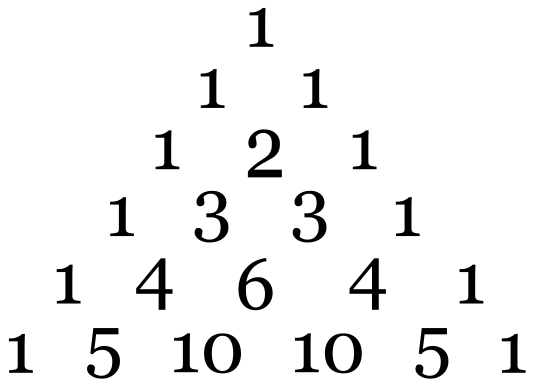
\includegraphics[width=0.4\textwidth]{pascal.png}
\caption{The first six rows of Pascal's triangle.}
\label{pascal}
\end{figure}

Now you might be wondering where I'm going with this. What do fun algebra
tricks have to do with counting combinations of items? The answer is that
the values of $\binom{n}{k}$ are \textit{precisely the coefficients of
these multiplied polynomials.} Let $n$ be 4, which corresponds to the last
polynomial we multiplied out. We can then compute all the combinations of
items taken from a group of four:
\[
\binom{4}{0}=1,
\binom{4}{1}=4,
\binom{4}{2}=6,
\binom{4}{3}=4,
\text{and}\ \binom{4}{4}=1.
\]
In other words, there is exactly \textit{one} way of taking no items out of
4 (you simply don't take any). There are \textit{four} ways of taking one
item out of 4 --- you could take the first, or the second, or the third, or
the fourth. There are \textit{six} ways of taking two items out of four;
namely:
\begin{center}
1. the first and second \\
2. the first and third \\
3. the first and fourth \\
4. the second and third \\
5. the second and fourth \\
6. the third and fourth
\end{center}
And so on.

Now in some ways we're on a bit of a tangent, since the fact that the
``n-choose-k" values happen to work out to be the same as the binomial
coefficients is mostly just an interesting coincidence. But what I really
want you to take notice of here --- and what Pascal's triangle makes plain
--- is the \textit{symmetry} of the coefficients. This surprises a lot of
students. What if I asked you which of the following numbers was greater:
$\binom{1000}{18}$ or $\binom{1000}{982}$? Most students guess that the
second of these numbers is far greater. In actual fact, though, they both
work out to $\frac{1000!}{18!982!}$ and are thus exactly the same. And in
the above example, we see that $\binom{4}{0}$ is equal to $\binom{4}{4}$,
and that $\binom{4}{1}$ is equal to $\binom{4}{3}$.

Why is this? Well, you can look back at the formula for $\binom{n}{k}$ and
see how it works out algebraically. But it's good to have an intuitive feel
for it as well. Here's how I think of it. Go back to the Davies kids and
the Wii. We said there were three different ways to choose 2 kids to play
on the Wii first after school. In other words, $\binom{3}{2} = 3.$ Very
well. But if you think about it, there must then also be three different
ways to \textit{leave out} exactly \textit{one} kid. If we change what
we're counting from ``combinations of players" to ``combinations of
non-players" --- both of which must be equal, since no matter what happens,
we'll be partitioning the Davies kids into players and non-players --- then
we see that $\binom{3}{1}$ must also be 3. 

And this is true across the board. If there are $\binom{500}{4}$ different
lineups of four movies, then there are the same number of lineups of 496
movies, since $\binom{500}{4} = \binom{500}{496}$. Conceptually, in the
first case we choose a group of four and show them, and in the second case
we choose a group of four and show \textit{everything but them.} 

Also notice that the way to get the greatest number of combinations of $n$
items is for $k$ to be half of $n$. If we have 100 books in our library,
there are a lot more ways to check out 50 of them then there are to check
out only 5, or to check out 95. Strange but true.

Lastly, make sure you understand the extreme endpoints of this phenomenon.
$\binom{n}{0}$ and $\binom{n}{n}$ are both always 1, no matter what
$n$ is. That's because if you're picking \textit{no} items, you have no
choices at all: there's only one way to come up empty. And if you're
picking \textit{all} the items, you also have no choices: you're forced to
pick everything.

\section{Summary}

Most of the time, counting problems all boil down to a variation of one of
the following three basic situations:

\begin{itemize}
\item $n^k$ --- this is when we have $k$ different things, each of which
is free to take on one of $n$ completely independent choices.
\item $n^{\underline{k}}$ --- this is when we're taking a sequence of $k$
different things from a set of $n$, but no repeats are allowed. (A special
case of this is $n!$, when $k=n$.)
\item $\binom{n}{k}$ --- this is when we're taking $k$ different things
from a set of $n$, but the order doesn't matter.
\end{itemize}

Sometimes it's tricky to deduce exactly which of these three situations
apply. You have to think carefully about the problem, and ask yourself
whether repeated values would be allowed, and whether it matters what order
the values appear in. This is often subtle.

\index{weightlifting}
As an example, suppose my friend and I work out at the same gym. This gym
has 18 different weight machines to choose from, each of which exercises a
different muscle group. Each morning, we each do a quick 30-minute workout
session divided into six 5-minute blocks, and we work with one of the
machines during each block, taking turns spotting each other. One day my
friend asks me, ``hey Stephen, have you ever wondered: how many different
workout routines are possible for us?"

I was, of course, wondering exactly that. But the correct answer turns out
to hinge very delicately on exactly what ``a workout routine" is. If we
could select any weight machine for any 5-minute block, then the answer is
$18^6$, since we have 18 choices for our first block, 18 choices for our
second, and so on. (This comes to 34,012,224 different routines, if you're
interested).

However, on further inspection, we might change our mind about this. Does
it make sense to choose the same machine more than once in a 30-minute
workout? Would we really complete a workout that consisted of ``1.Biceps
2.Abs, 3.Pecs, 4.Biceps, 5.Biceps, 6.Biceps?" If not (and most trainers
would probably recommend against such monomaniacal approaches to excercise)
then the real answer is only $18^{\underline{6}}$, since we have 18 choices
for our first block, and then only 17 for the second, 16 for the third,
\textit{etc.} (This reduces the total to 13,366,080.)

But perhaps the phrase ``a workout routine" means something different even
than that. If I tell my physical therapist what ``my workout routine"
consisted of this morning, does he really care whether I did triceps first,
last, or in the middle? He probably only cares about \textit{which}
machines (and therefore which muscle groups) I worked out that morning, not
what order I did them in. If this is true, then our definition of a workout
routine is somewhat different than the above. It's no longer a consecutive
sequence of machine choices, but rather a \textit{set} of six machine
choices. There would only be $\binom{18}{6}$ of those, or a mere 18,564. So
as you can see, the answer radically depends on the precise interpretation
of the concepts, which means that to successfully do combinatorics, you
have to slow down and think very carefully.
